\subsubsection{Demonstrators}

\TOWRITE{SL}{include the other demonstrators and emphasise links to rest of the project}




\paragraph{Demonstrator: Training and education of the next generation
  computationalists} --- We will produce a series of interactive books
that can be read, executed, modified and explored within the
\TheProject VREs, targetting Biology, Physics, Maths and Engineering
students to demonstate the power of the approach and to train future
scientists and engineers to embrace and exploit these advances in
computational methodology (\taskref{dissem}{ibook}). We will also
create additional materials for teachers at all levels to help them
act as multipliers and disseminate the advances developed here widely~(\taskref{dissem}{project-intro}).
\TOWRITE{SL}{Stephen (?) I have added a first draft for other
  demonstrators (above) - have we got more?, Hans}

\begin{figure}
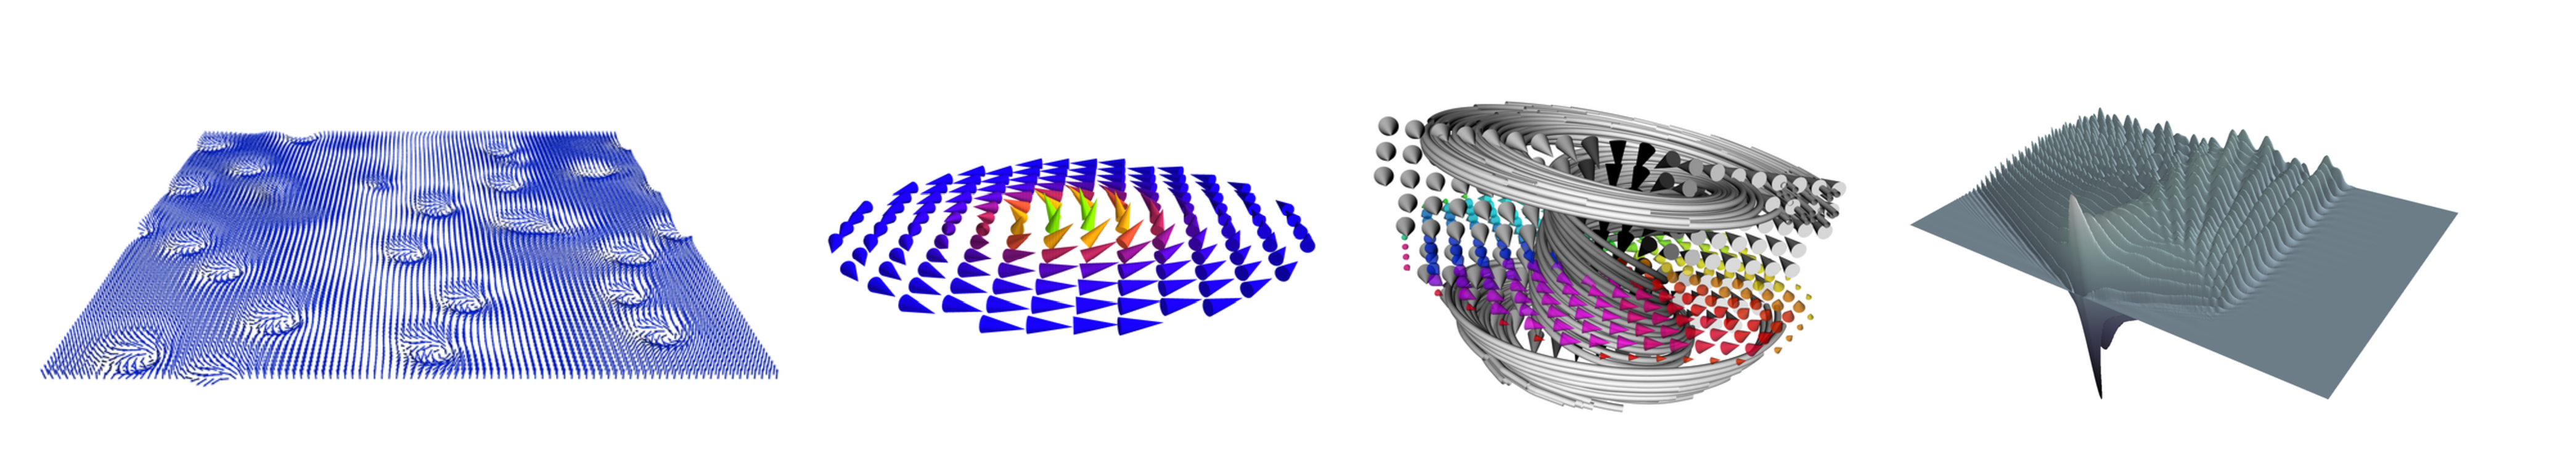
\includegraphics[width=1.0\textwidth]{Pictures/micromagnetic-and-3d-vis-4x1.pdf}
\caption{\label{fig:3d-plots} A selection of typical visualisation patterns often required in science and engineering. From left to right: a 3d vector field on a 2d domain, a 3d vector field coloured with another scalar field on a 2d domain, a 3d vectorfield on a 3d domain with streamlines, and scalar field plotted on a 2d domain.}
\end{figure}

\paragraph{Demonstrator: Micromagnetic VRE}
\label{sec:introduction-micromagnetic-vre-demonstrator}
--- Micromagnetics is a continuum theory description of the behaviour of
the magnetisation vector field at length scales of the order of
micrometers and below. It is widely used in the research and
development of magnetic data storage media and devices, for magnetic
sensing, permanent magnets and healthcare applications such as cancer
treatment and diagnostics. The mathematical model is a time dependent
nonlinear partial differential equation with multiple length and time
scales in the problem, and solution strategies are based on finite
difference and finite element space discretisations and sophisticated
numerical solution of the equations. As in many other applied research fields,
the groups carrying out the simulations are often not the code
developers, nor have they extensive computational background. More
commonly, these are material scientists, engineers and physicists that
use the simulation to interpret their experiments and support their
device design planning. Industrial users include Seagate, Hitachi,
TDK, Samsung, Bosch and Toyota.

Figure~\ref{fig:3d-plots} shows magnetisation vector fields obtained
in typical micromagnetic studies. They relate, from left to
right, to a set of interacting magnetic skyrmions in a thin flim, a
vortex in a thin Nickel film, a vortex in a half-sphere geometry, and
the propagation of magnetic excitations in a 1d-system.

Here, we will use the \TheProject components to put
together a in micromagnetic VRE to (i) demonstrate the power of the
approach in a concrete applied research setting, (ii) exploit that
experience to evaluate the real value of the structure of this VRE and
\TheProject to a large and diverse set of end-users. In more detail, we will embed the most popular micromagnetic
simulation software (Object Oriented MicroMagnetic Framework
\cite{OOMMF-url}) within a micromagnetic VRE, complement this with
value-adding features, develop a number of executable
documents inside this VRE that act as tutorials and documentation,
disseminate the software and documents as open source and through
workshops for the micromagnetic community.  

We have chosen the OOMMF simulation package as the target tool because
it is a somewhat typical representative of computational software:
computation is driven through a text-based configuration file, data
files are produced, and later processed, then figures are created from
the processed data; leaving the scientist with the burden to link all
these elements together. The benefits of moving to the integrated
notebook workflow (see Section~\ref{sec:jupyter}) are
substantial. Furthermore, OOMMF is widely used (over 1800 recorded
publications \cite{OOMMF-citations-url}) and thus provides benefit to
an active and substantial community, who in return will provide plenty
of feedback.

We evaluate the value of this demonstrator
(\taskref{social-aspects}{oommf-nb-evaluation}), immediately feeding
results back into the \TheProject work. This will also
be a case study for the sustainability of the approach and tool beyond
the life time of this H2020 project.

